\include{template}
%\cfoot{} %% if no page number is needed

\begin{document}

\begin{header}
Chapitre 1 -- Corps purs et mélanges
\end{header}

\section{Rappels}

\begin{figure}[h]
\center
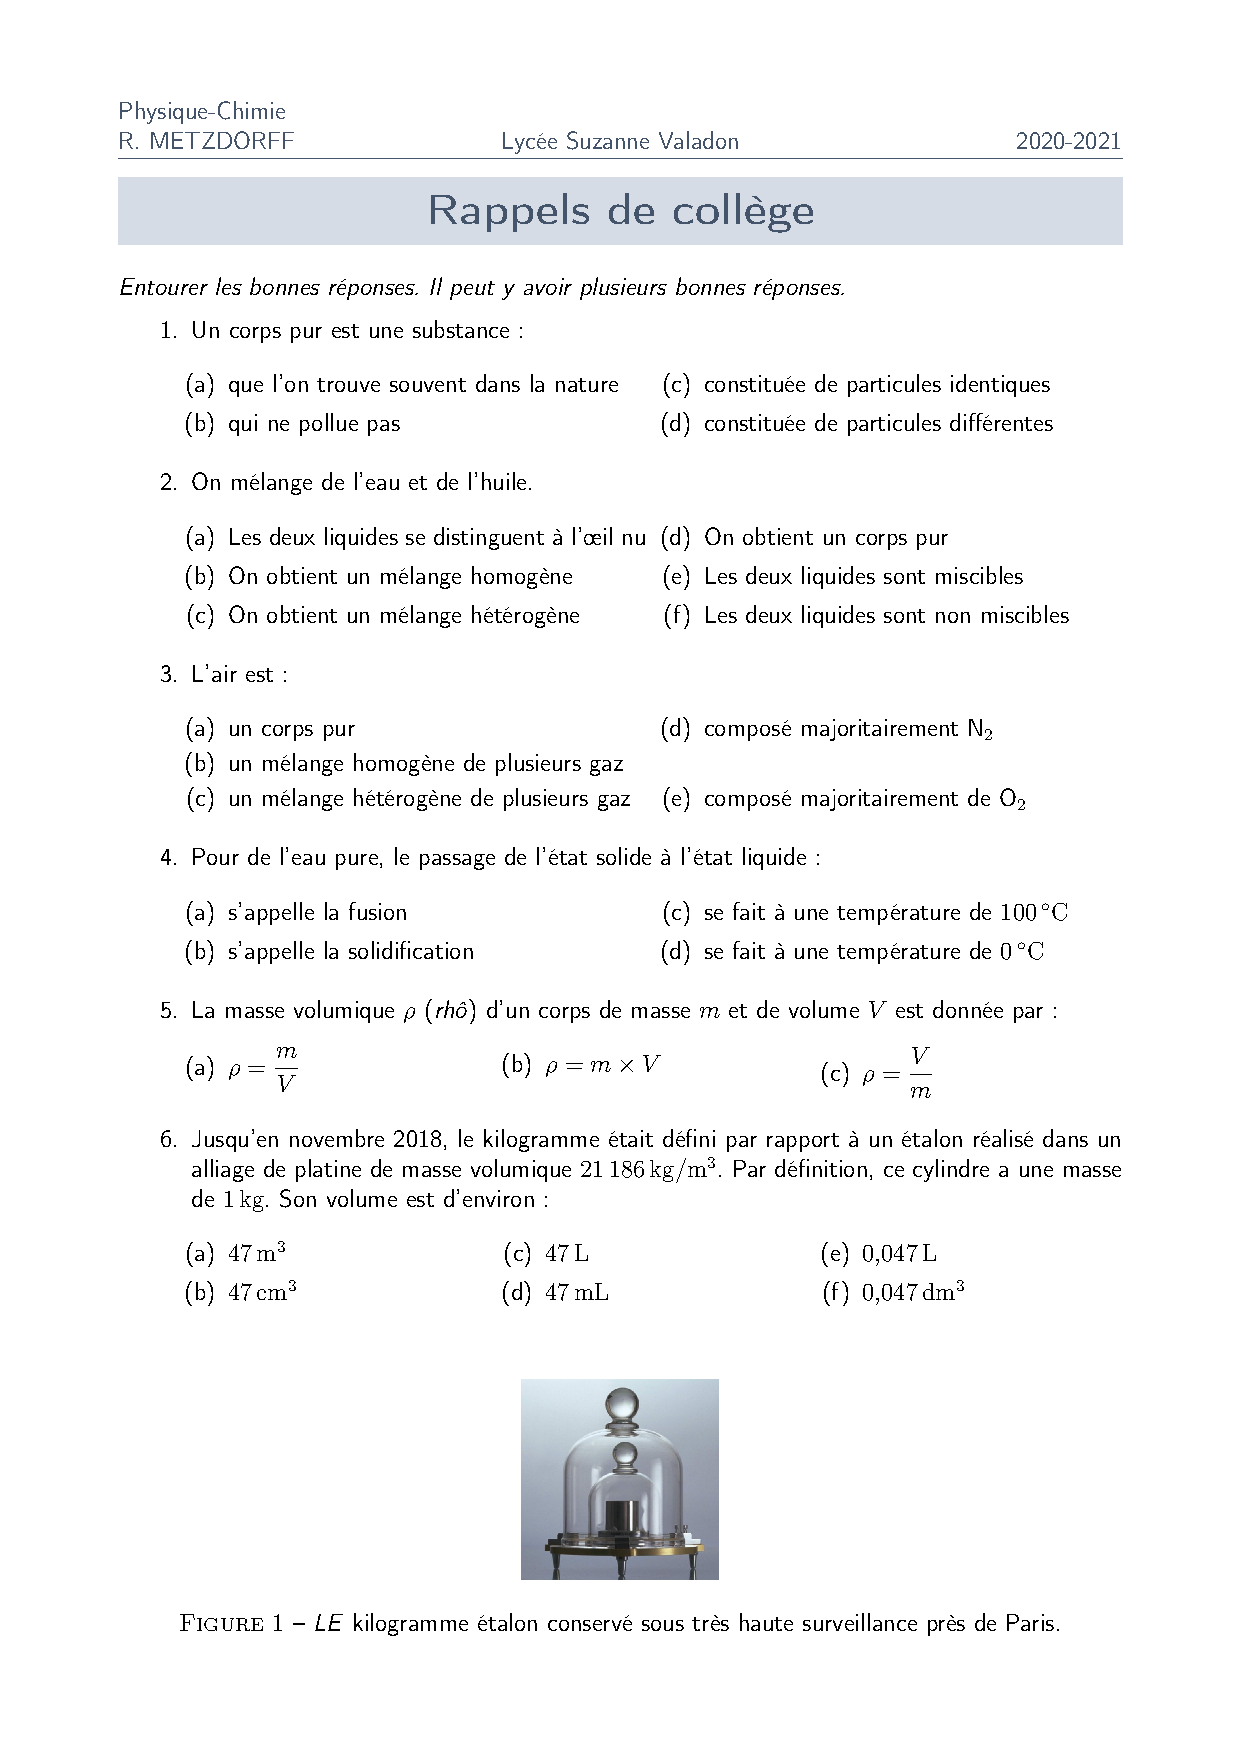
\includegraphics[scale=0.5]{chap1_qcm_rappels.pdf}
\caption{QCM donné aux élèves avant d'entamer le chapitre : évaluation diagnostique.}
\end{figure}

Correction : 1-c ; 2-a,c,f ; 3-b,d ; 4-a,d ; 5-a ; 6-b,d,e,f.

\begin{prior}
Distribuer le QCM rappel :
\emph{Je vous distribue le QCM, vous avez \unit{10}{\minute} pour le compléter (ou jusqu'à la fin du cours et à terminer à la maison : noter dans l'agenda... Je vérifierai la prochaine fois).
Il ne sera pas ramassé, nous le corrigerons ensemble.}

\noindent
\emph{Correction :}
Pour chaque question, estimer le pourcentage de réponses justes dans la classe et identifier les concepts qui ont posé problème.
Pour la question 5, on commence la fiche \emph{Outils mathématiques}.
Durée estimée de la correction : \unit{15}{\minute}.
\end{prior}

\section{Corps purs et mélanges}
\label{sec:corps_purs_melanges}

\begin{figure}[h]
\center
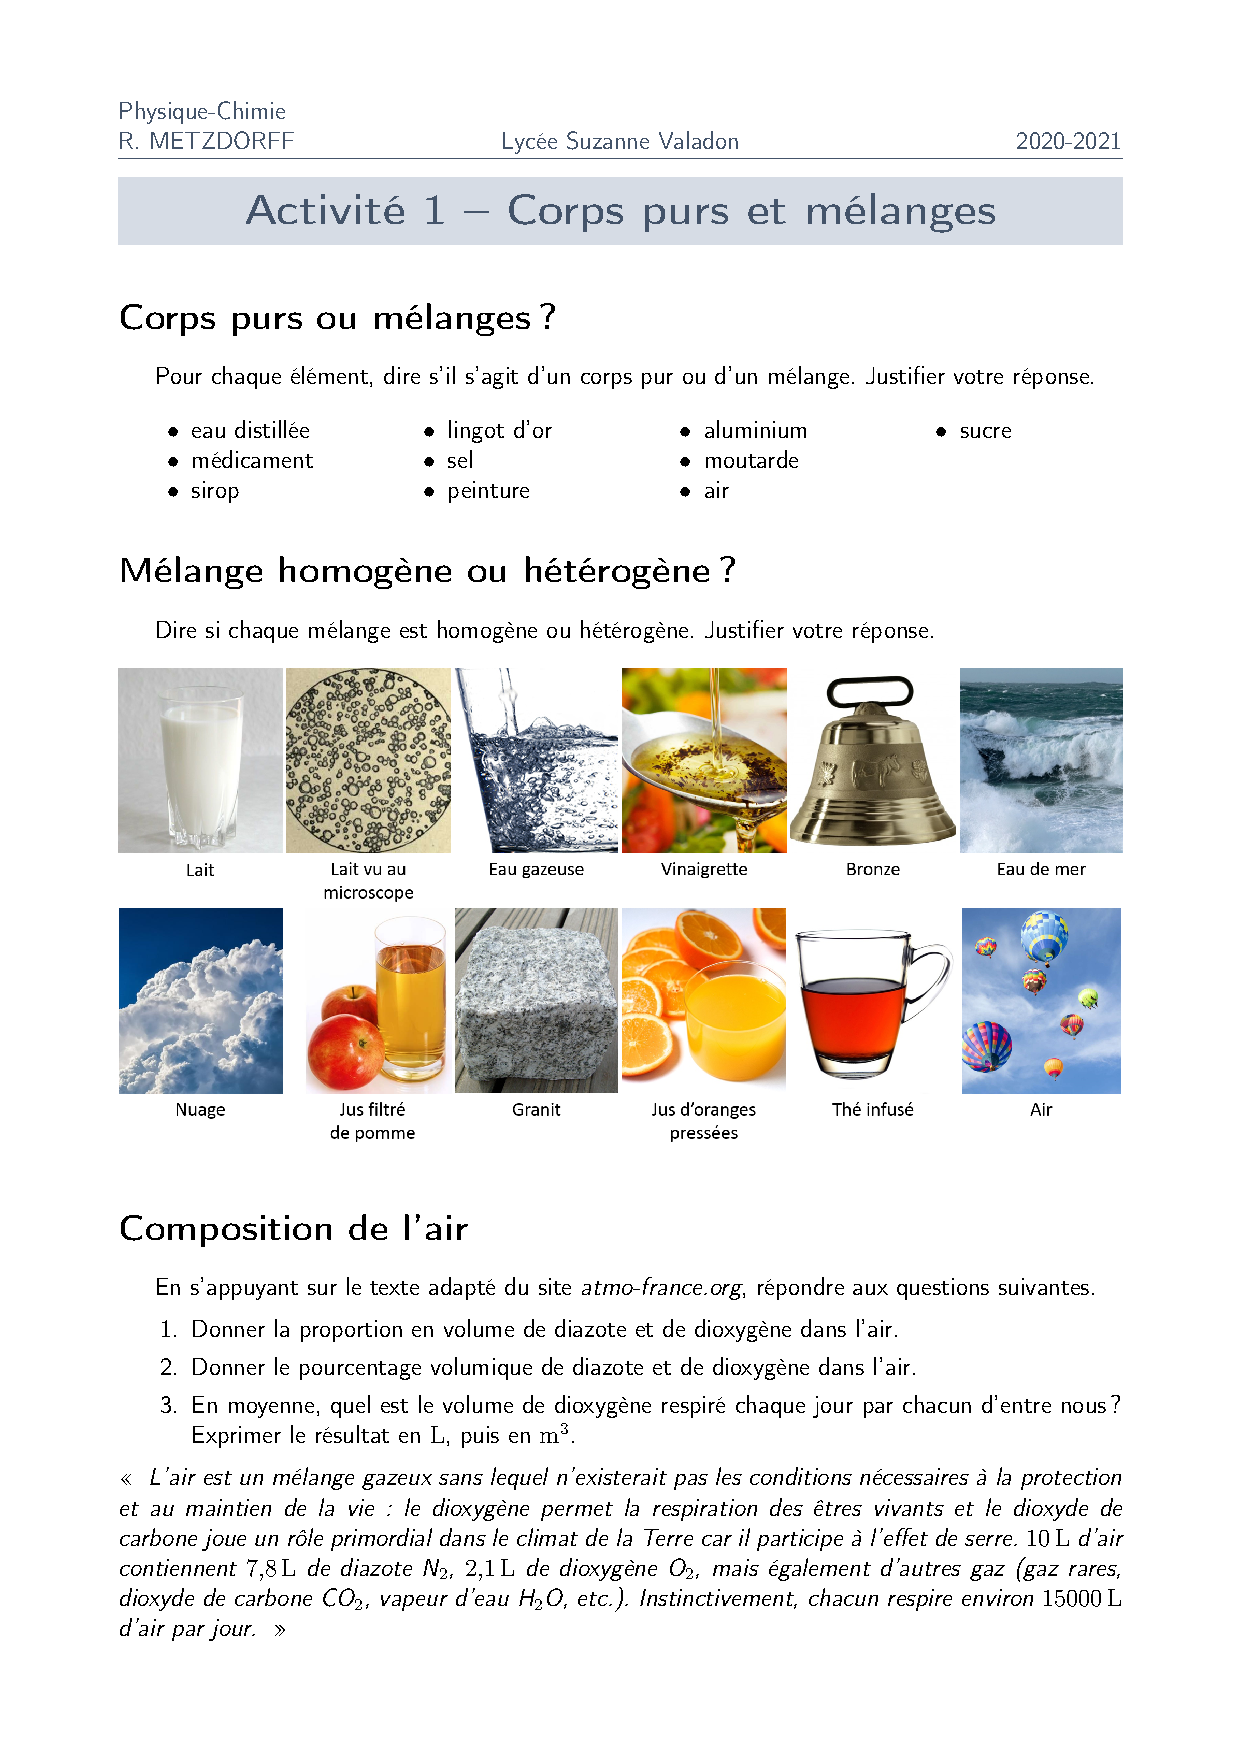
\includegraphics[scale=0.5]{chap1_act1.pdf}
\caption{Activité 1 support de cours pour la section~\ref{sec:corps_purs_melanges}.}
\end{figure}

\subsection{Corps purs ou mélange ?}

\begin{prior}
Distribuer l'activité 1.
\emph{Je vous distribue la première activité, nous allons la faire ensemble, puis nous trouverons une définition de ces deux termes.}
Pour chaque point, je fais un sondage dans la classe.
\emph{On démarre l'activité 1, vous allez me dire si chacun de ces éléments est un corps pur ou un mélange.
On vote à main levée et je note la réponse qui l'emporte.}
On écrit les définitions : espèce chimique, corps pur et mélange.
Temps estimé : \unit{10-15}{\minute}.
\end{prior}

\begin{exemple}
\emph{correction de l'activité 1.}
\center
\begin{tabular}{c|c}
\textbf{Corps pur} & \textbf{Mélange} \\
\hline
Eau distillée & Médicament \\
Lingot d'or   & Sirop \\
Sel           & Peinture \\
Aluminium     & Moutarde \\
Sucre         & Air
\end{tabular}
\end{exemple}

\begin{definition}
Un \textbf{corps pur} est composé d'une seule espèce chimique.

\noindent
Un \textbf{mélange} est composé de plusieurs espèces chimiques.
\end{definition}

\begin{definition}
Une \textbf{espèce chimique} est un ensemble d'entités chimiques (atomes, ions, molécules, etc.) \textit{identiques}.
Elle est représentée par un symbole chimique.
\end{definition}

\begin{exemple}
L'aluminium Al, l'ion chlorure $\chlorure$, l'eau $\eau$.
\end{exemple}

\begin{slide}
\textbf{Le sucre -- Sacharose}

\noindent
\textcolor{green_f}{Revenir sur les exemples et donner les espèces chimiques associées.}
\end{slide}


\subsection{Mélange homogène ou hétérogène ?}

\begin{prior}
\emph{Sur votre cahier de brouillon, vous avez \unit{5}{\minute} pour classer les différents mélanges représentés en photo dans deux colonnes : homogènes ou hétérogène.
Justifiez votre réponse}
\end{prior}

\begin{exemple}
\emph{correction de l'activité 1.}
\center
\begin{tabular}{c|c}
\textbf{Mélange homogène} & \textbf{Mélange hétérogène} \\
\hline
Lait                & Lait vu au microscope \\
Bronze              & Eau gazeuse \\
Eau de mer          & Vinaigrette \\
Jus filtré de pomme & Nuages \\
Thé infusé          & Granit \\
Air                 & Jus d'oranges pressées
\end{tabular}
\end{exemple}

Après agitation, les constituants d'un mélange homogène sont indiscernables à l'œil nu.
Dans un mélange hétérogène, on distingue au moins deux constituants à l'œil nu même après agitation.
(on peut prendre l'exemple du sirop pour insister sur l'aspect agitation)

\begin{definition}
Deux liquides \textbf{miscibles} forment un mélange homogène.
Deux liquides \textbf{non-miscibles} forment un mélange hétérogène.
\end{definition}

\subsection{Représentation microscopique}

\begin{prior}
On fait le corps pur ensemble le corps pur pour l'exemple.
\emph{Sur votre cahier de brouillon, en représentant les particules des différentes espèces chimiques par des ronds de différentes couleurs, dessinez le contenu de deux verres contenants respectivement un mélange de deux liquides miscibles et un mélange de deux liquides non-miscibles.}
\end{prior}

\section{Identification d'espèces chimiques}

\begin{figure}[h]
\center
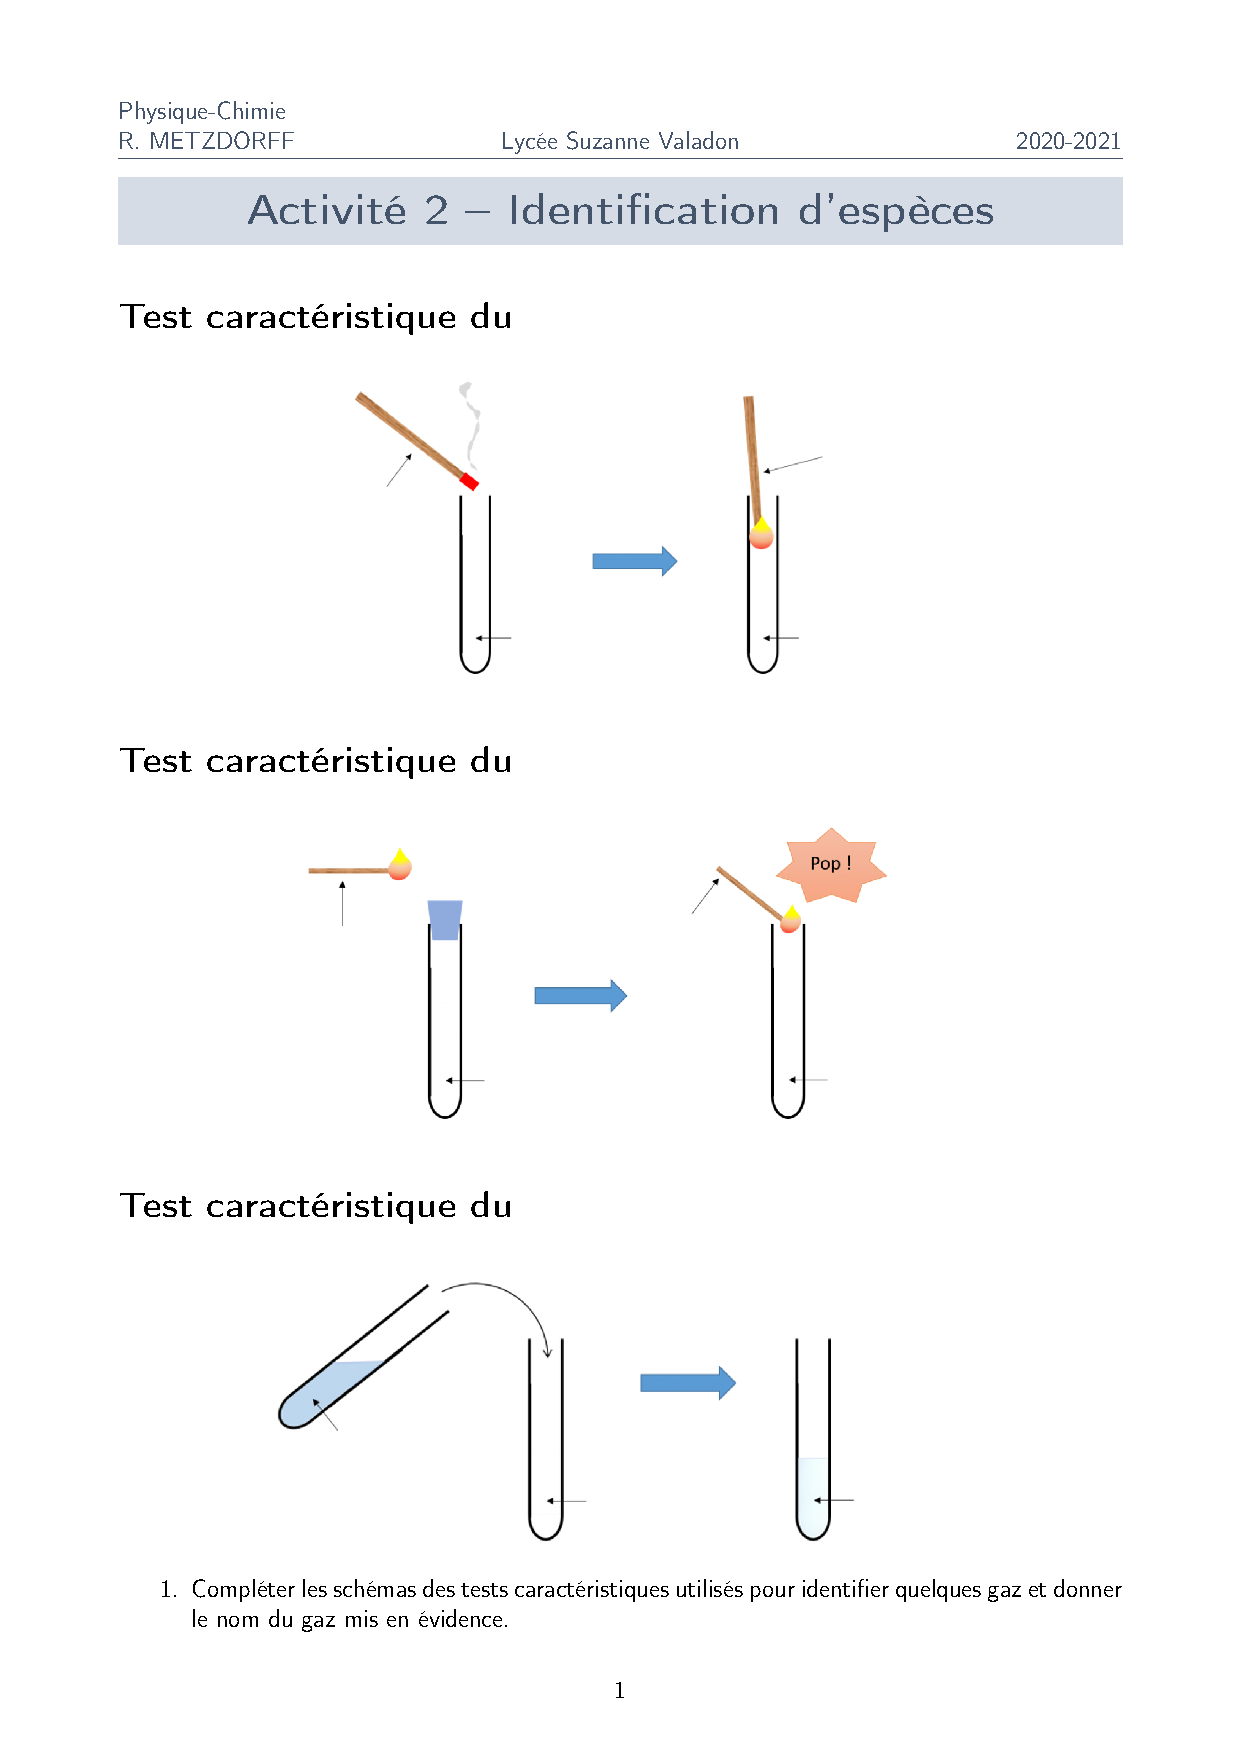
\includegraphics[page=1,scale=0.4]{chap1_act2.pdf}
\includegraphics[page=2,scale=0.4]{chap1_act2.pdf}
\caption{Activité 2 sur l'identification d'espèces chimiques.}
\end{figure}

\subsection{Tests caractéristiques chimiques}

\begin{itemize}
\item[•] Test d'identification de l'eau : \href{https://tinyurl.com/thbmmcd}{https://tinyurl.com/thbmmcd}
\item[•] Test d'identification du dioxygène : \href{https://tinyurl.com/y4y7elaf}{https://tinyurl.com/y4y7elaf}
\item[•] Test d'identification du dihydrogène : \href{https://tinyurl.com/y6a4kqw6}{https://tinyurl.com/y6a4kqw6}
\item[•] Test d'identification du dioxyde de carbone : \href{https://tinyurl.com/lef4pb5}{https://tinyurl.com/lef4pb5}
\end{itemize}

\begin{prior}
En se basant sur les vidéos ou sur les expériences réalisées par le professeur : \emph{Chacun pour soi, vous avez 2 min pour compléter au crayon de papier le schéma correspondant à l'expérience réalisée sur l'activité 2.}
Insister sur l'importance du schéma.
Deux types de schéma : schéma d'une expérience, schéma d'un montage.
Évoquer le schéma narratif.
\end{prior}

En présence de dioxygène, un buchette incandescente se rallume.

Quand on approche une flamme du dihydrogène, une détonation se produit.

En présence de dioxyde de carbone, l'eau de chaux se trouble.

En présence d'eau, le sulfate de cuivre devient bleu.

\subsection{Propriétés physiques}

\begin{slide}
\textbf{Propriétés physico-chimiques.}
\end{slide}

Les corps purs ont des propriétés physiques qui permettent de les identifier :
\begin{itemize}
\item[•] la masse volumique ;
\item[•] les températures de changement d'état ;
\item[•] la solubilité ;
\item[•] l'indice de réfraction ;
\item[•] etc.
\end{itemize}

\begin{prior}
Faire la question 2 de l'activité 2 : on pose la question aux élèves et on écrit les valeurs en rouge.
Il faut les connaitre !
\end{prior}

\begin{prior}
Faire les questions 3 et 4 de l'activité 2 : \emph{Vous avez 5 minutes pour répondre aux questions 3 et 4 de l'activité 2 sur votre cahier de brouillon.}
\end{prior}

\begin{definition}
La \textbf{masse volumique} $\rho$ d'une substance de masse $m$ et de volume $V$ s'exprime par :
\begin{equation}
\rho = \frac{m}{V}.
\nonumber
\end{equation}
\end{definition}
Rq : unités, dépend de la température.

\begin{definition}
La \textbf{densité} $d$ d'un solide ou d'un liquide de masse volumique $\rho$ est définie par rapport à l'eau :
\begin{equation}
d = \frac{\rho}{\rho_\mathrm{eau}}.
\nonumber
\end{equation}

La densité d'un gaz est définie par rapport à l'air :
\begin{equation}
d = \frac{\rho}{\rho_\mathrm{air}}.
\nonumber
\end{equation}
\end{definition}
Rq : Attention aux unités !

\begin{prior}
Faire les questions 5 et 6 de l'activité.
\end{prior}

\begin{figure}[h]
\center
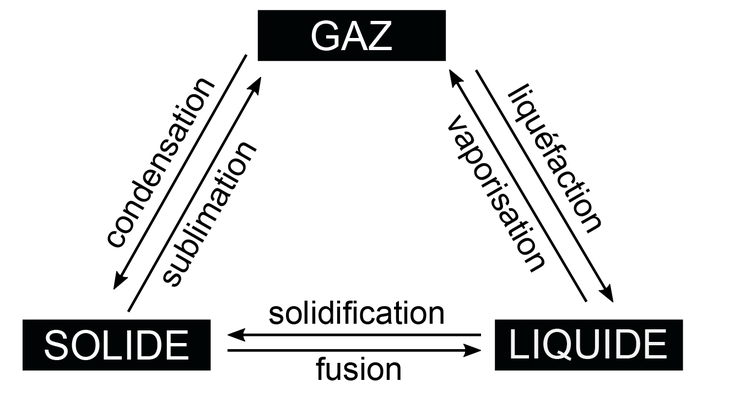
\includegraphics[scale=1]{images/changements_d_etat.jpg}
\end{figure}

\begin{prior}
On utilise la vidéo \href{https://tinyurl.com/yxmtwo32}{https://tinyurl.com/yxmtwo32}.
La passer en entier vitesse doublée en la présentant comme la vidéo la plus folle de tous les temps.
Indiquer en fonction du temps les états sous lesquels se trouve l'eau en ajoutant des balises : sortie du congélateur, début de la vidéo (les glaçons commencent à fondre), fin de la vidéo puis plus loin...
Je trace le graphique en indiquant les balises et ils complètent.
\emph{Sur le graphe indiquer sous quelle\cdot s forme\cdot s l'eau est présente.}
\emph{Tracer l'évolution de la température.}
\emph{Que se passe-t-il si l'eau est salée ?}
\end{prior}

\begin{figure}[h]
\center
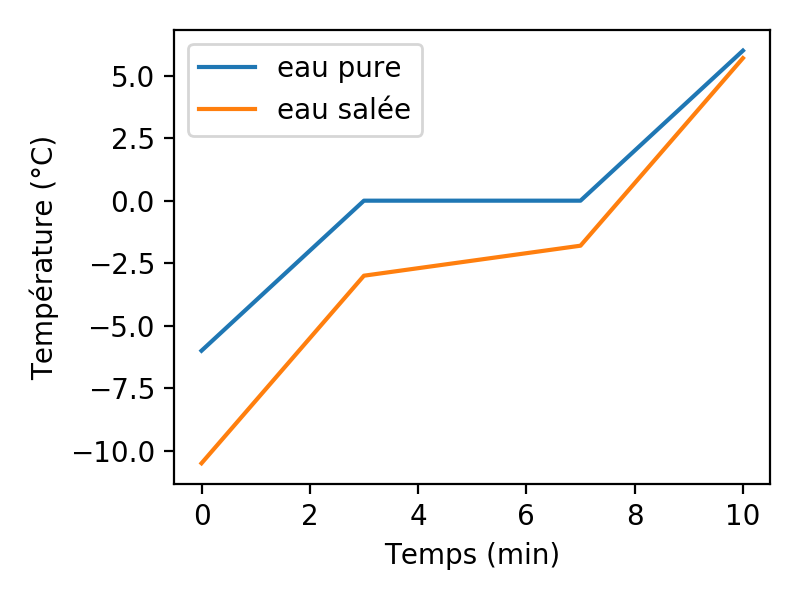
\includegraphics[scale=0.75]{images/fusion.png}
\caption{Suivis thermométriques de la fonte de glace d'eau pure et de glace d'eau salée.}
\end{figure}

\begin{prior}
Faire la question 7 de l'activité 2.
\end{prior}

\begin{definition}
Un corps pur \textbf{change d'état à température constante}.
Ce n'est pas le cas pour un mélange.
\end{definition}

\begin{slide}
\textbf{Mesure de la température de fusion –- Le banc Kofler}
\end{slide}

\subsection{Chromatographie}

\begin{prior}
On utilise la vidéo \href{https://tinyurl.com/y6neowtg}{https://tinyurl.com/y6neowtg}.
Montrer la vidéo à partir de \unit{30}{\second} jusqu'à l'introduction dans la cuve.
\emph{Sur votre cahier de brouillon, vous avez \unit{3}{\minute} pour formuler une hypothèse sur ce qui va se passer.}
\emph{En groupe, vous avez \unit{5}{\minute} pour vous mettre d'accord sur une hypothèse.}
On regarde la vidéo.
\emph{Sur votre cahier de brouillon, \unit{5}{\minute} pour interpréter.}
On fait le bilan.
\end{prior}

\begin{definition}
La chromatographie sur couche mince (CCM) permet de \textbf{séparer} et \textbf{identifier} les espèces chimiques présentes dans un mélange.
\end{definition}
Rq : pour un éluant et un support donnés, une espèce chimique migre de la même façon qu'elle soit pure ou présente dans un mélange.

\begin{figure}[h]
\center
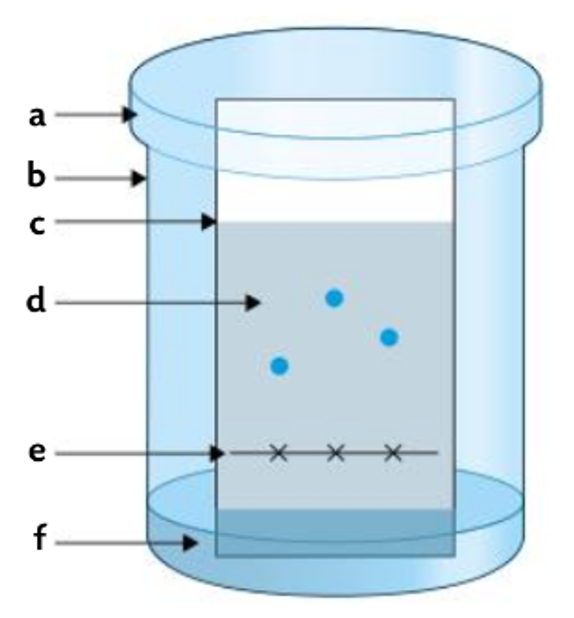
\includegraphics[scale=0.5]{images/ccm_schema.png}
\caption{Schéma du montage expérimental utilisé pour réaliser une CCM.
a : coupelle, b : cuve, c : front de l'éluant, d : phase stationnaire, e : ligne de dépôt et f : phase mobile (éluant).}
\end{figure}



\section{Composition d'un mélange}

\subsection{Composition volumique : l'air}

\begin{prior}
\emph{Quelqu'un lit le texte de l'activité 1.
Sur votre cahier de brouillon, vous avez \unit{2}{\minute} pour répondre aux deux premières questions.
Alors, comment est-ce qu'on calcule la proportion volumique ?}
Pour la question 3, on continue la fiche outils \emph{Outils mathématiques} sur les unités 1D et 3D.
Les élèves doivent se familiariser avec le volume que représente le litre et le mètre cube.
\end{prior}

Le pourcentage volumique de diazote dans l'air est \unit{78}{\%}.
Le pourcentage volumique de dioxygène dans l'air est \unit{21}{\%}.
Chacun respire \unit{3150}{\liter} de dioxygène par jour, soit \unit{3{,}15}{\meter^3}.

\begin{definition}
La \textbf{proportion en volume} d'une espèce E dans un mélange s'exprime comme le quotient du volume de cette espèce $V_\mathrm{E}$ par le volume total du mélange $V_\mathrm{tot}$ :
\begin{equation}
\frac{V_\mathrm{E}}{V_\mathrm{tot}}.
\nonumber
\end{equation}
Si elle est exprimée en pourcent, on parle de \textbf{pourcentage volumique}.
\end{definition}
Pour calculer la proportion en volume, il faut que les deux volumes aient la même unité !
La proportion en volume (le pourcentage volumique) d'une espèce dans un mélange ne peut être supérieur à 1 (à \unit{100}{\%}) !

\begin{definition}
Pour passer d'une proportion en volume à un pourcentage massique, on multiplie la  proportion en volume par cent.
\end{definition}

\subsection{Composition massique}

\end{document}